\begin{question}
    
    \begin{enumerate}[label=\textbf{\alph*})]
        \item 
        
        \begin{minipage}{\linewidth}
            \centering
            
            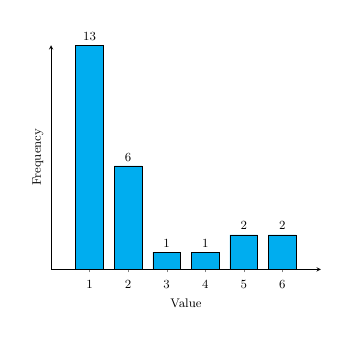
\begin{tikzpicture}[font=\small, scale=0.5]
                \begin{axis}[
                  ybar,
                  bar width=20pt,
                  xlabel={Value},
                  ylabel={Frequency},
                  ymin=0,
                  ytick=\empty,
                  xtick=data,
                  axis x line=bottom,
                  axis y line=left,
                  enlarge x limits=0.2,
                  symbolic x coords={1,2,3,4,5,6},
                  xticklabel style={anchor=base,yshift=-\baselineskip},
                  nodes near coords={\pgfmathprintnumber\pgfplotspointmeta}
                ]
                  \addplot[fill=cyan] coordinates {
                    (1,13)
                    (2,6)
                    (3,1)
                    (4,1)
                    (5,2)
                    (6,2)
                  };
                \end{axis}
            \end{tikzpicture}

            \hspace{0.5cm}

            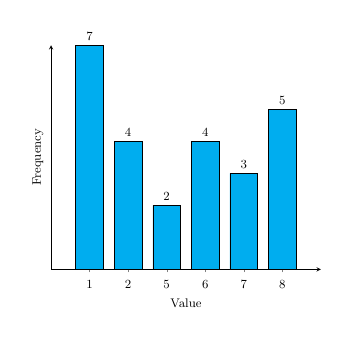
\begin{tikzpicture}[font=\small, scale=0.5]
                \begin{axis}[
                  ybar,
                  bar width=20pt,
                  xlabel={Value},
                  ylabel={Frequency},
                  ymin=0,
                  ytick=\empty,
                  xtick=data,
                  axis x line=bottom,
                  axis y line=left,
                  enlarge x limits=0.2,
                  symbolic x coords={1,2,5,6,7,8},
                  xticklabel style={anchor=base,yshift=-\baselineskip},
                  nodes near coords={\pgfmathprintnumber\pgfplotspointmeta}
                ]
                  \addplot[fill=cyan] coordinates {
                    (1,7)
                    (2,4)
                    (5,2)
                    (6,4)
                    (7,3)
                    (8,5)
                  };
                \end{axis}
            \end{tikzpicture}

            \hspace{0.5cm}
            
            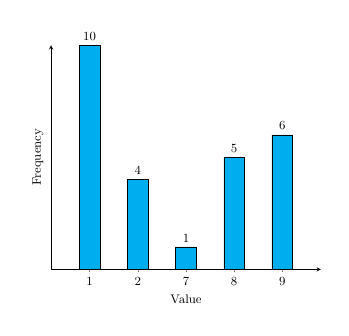
\begin{tikzpicture}[font=\small, scale=0.5]
                \begin{axis}[
                  ybar,
                  bar width=15pt,
                  xlabel={Value},
                  ylabel={Frequency},
                  ymin=0,
                  ytick=\empty,
                  xtick=data,
                  axis x line=bottom,
                  axis y line=left,
                  enlarge x limits=0.2,
                  symbolic x coords={1,2,7,8,9},
                  nodes near coords={\pgfmathprintnumber\pgfplotspointmeta}
                ]
                  \addplot[fill=cyan] coordinates {
                    (1,10)
                    (2,4)
                    (7,1)
                    (8,5)
                    (9,6)
                  };
                \end{axis}
            \end{tikzpicture}
        \end{minipage}
 
        \item 


    \end{enumerate}
\end{question}